\documentclass[12pt]{article}
\usepackage{amsthm,amssymb,amsmath,amsfonts}
\usepackage[a4paper, top=25mm, bottom=30mm, left=25mm, right=25mm]{geometry}
\usepackage[pagebackref=false,colorlinks,linkcolor=black,citecolor=black]{hyperref}
\usepackage[nameinlink]{cleveref}
 \AtBeginDocument{%
    \crefname{equation}{برابری}{equations}%
    \crefname{chapter}{فصل}{chapters}%
    \crefname{section}{بخش}{sections}%
    \crefname{appendix}{پیوست}{appendices}%
    \crefname{enumi}{مورد}{items}%
    \crefname{footnote}{زیرنویس}{footnotes}%
    \crefname{figure}{شکل}{figures}%
    \crefname{table}{جدول}{tables}%
    \crefname{theorem}{قضیه}{theorems}%
    \crefname{lemma}{لم}{lemmas}%
    \crefname{corollary}{نتیجه}{corollaries}%
    \crefname{proposition}{گزاره}{propositions}%
    \crefname{definition}{تعریف}{definitions}%
    \crefname{result}{نتیجه}{results}%
    \crefname{example}{مثال}{examples}%
    \crefname{remark}{نکته}{remarks}%
    \crefname{note}{یادداشت}{notes}%
    \crefname{observation}{مشاهده}{observations}%
    \crefname{algorithm}{الگوریتم}{algorithms}%
    \crefname{cproof}{برهان}{cproofs}%
}

\usepackage{tikz}
\usepackage{graphicx}
\usepackage{color}

\usepackage{setspace}
\doublespacing

\usepackage{titletoc}
\usepackage{tocloft}
\usepackage{enumitem}

\usepackage{algorithm}
% \usepackage[noend]{algpseudocode}
\usepackage[noend]{algorithmic}
\renewcommand{\algorithmicrequire}{\textbf{Input:}}
\renewcommand{\algorithmicensure}{\textbf{Output:}}

\usepackage{tabularx}
\makeatletter
\newcommand{\multiline}[1]{%
  \begin{tabularx}{\dimexpr\linewidth-\ALG@thistlm}[t]{@{}X@{}}
    #1
  \end{tabularx}
}
\makeatother

\usepackage{float}
\usepackage{verbatim}
\makeindex
\usepackage{sectsty}
\usepackage{xepersian}
\SepMark{-}
\settextfont[Scale=1.2,Path=fonts/,BoldFont=B Nazanin Bold.ttf]{B Nazanin.ttf}
\setlatintextfont{Times New Roman}
\renewcommand{\labelitemi}{$\bullet$}

\theoremstyle{definition}
\newtheorem{definition}{تعریف}[section]
\newtheorem{remark}[definition]{نکته}
\newtheorem{note}[definition]{یادداشت}
\newtheorem{example}[definition]{نمونه}
\newtheorem{question}[definition]{سوال}
\newtheorem{remember}[definition]{یاداوری}
\newtheorem{observation}[definition]{مشاهده}
\theoremstyle{theorem}
\newtheorem{theorem}[definition]{قضیه}
\newtheorem{lemma}[definition]{لم}
\newtheorem{proposition}[definition]{گزاره}
\newtheorem{corollary}[definition]{نتیجه}
\newtheorem*{cproof}{برهان}



\begin{document}
\fontsize{12pt}{14pt}\selectfont

\begin{minipage}{0.1\textwidth}

\end{minipage}%
\hfill%
\begin{minipage}{0.6\textwidth}\centering
\fontsize{10pt}{10pt}\selectfont
به نام خداوند \\
تئوری یادگیری ماشین \\
دکتر سیدصالحی\\
جلسه سوم
 \\
\vspace{0.25cm}
\begingroup
\fontsize{8pt}{8pt}\selectfont
دانشکده ریاضی و علوم کامپیوتر \\
اسفند ماه 1402\\
\endgroup
\end{minipage}%
\hfill%
\begin{minipage}{0.1\textwidth}
\end{minipage}

\vspace{0.5cm}

\noindent\rule{\textwidth}{1pt}

\section*{$Gaussian\:discriminant\:analysis$}
مثالی که جلسه قبل بررسی کردیم یک مثال از یک دسته از مدل ها بود به نام $GDA$. تو $GDA$ ما فرضی که میکنیم که توضیع های $conditional$ ما یه سری توضیع نرمال هستند و اینکه $prior$ روی کلاس های ما برنولی هست.(فرض ما حالت دوکلاس مساله است.)
\begin{figure}[h]
  \centering
  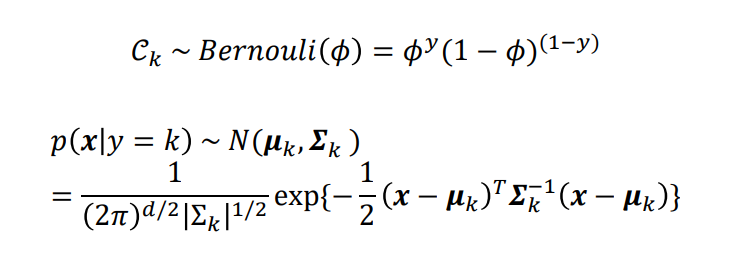
\includegraphics[width=0.6\textwidth]{figs/1.png}
  \label{1}
\end{figure}

\[ 
P(X=x|Y=1) = \frac{1}{(2\pi)^{\frac{n}{2}}|\Sigma_1|^{\frac{1}{2}}} \exp \left( -\frac{1}{2}(x-\mu_1)^T \Sigma_1^{-1} (x-\mu_1) \right)
\]
\[ 
P(X=x|Y=0) = \frac{1}{(2\pi)^{\frac{n}{2}}|\Sigma_0|^{\frac{1}{2}}} \exp \left( -\frac{1}{2}(x-\mu_0)^T \Sigma_0^{-1} (x-\mu_0) \right)  
\]
ما تا الآن $prior$ کلاس ها را به صورت فرض شده در نظر گرفتیم ولی الآن کمی مدل بهتری میتونیم اتخاذ کنیم. یک تابع $likelihood$ تشکیل میدیم با فرض $iid$ بودن سمپل ها:

\begin{align*}
\ell(\phi, \mu_0, \mu_1, \Sigma_1, \Sigma_2) &= \log \prod_{i=1}^{N} p(x^{(i)}, y^{(i)}; \phi, \mu_0, \mu_1, \Sigma_0, \Sigma_1) \\
&= \log \prod_{i=1}^{N} p(x^{(i)}| y^{(i)}, \mu_0, \mu_1, \Sigma_0, \Sigma_1) p(y^{(i)}; \phi)
\end{align*}
با ماکزیمم کردن $\ell$ با توجه به پارامترها، تخمین $likelihood$ پارامترها را پیدا می کنیم.

\begin{itemize}
    \item برای به حداکثر رساندن $\ell(\cdot)$ با توجه به پارامترها، مشتق $\ell(\cdot)$ را می‌گیریم، مشتق را برابر 0 قرار می‌دهیم و سپس مقادیر پارامترهایی که عبارت $\ell(\cdot)$ را به حداکثر می‌رساند را حل می‌کنیم. این تخمین حداکثر احتمال $\phi$ را به دست می‌دهد.

    توضیح شهودی در مورد مقدار \( \phi \) برای به حداکثر رساندن $Likelihood$ به شرح زیر است. به یاد بیاورید که \( \phi \) تخمین احتمال \( y \) برابر با ۱ است. در مثال خاص ما، این شانس که بیمار بعدی با تومور بدخیم به مطب پزشک شما می‌رود با \( \phi \) نشان داده می‌شود. احتمال شیر آمدن در پرتاب سکه، کسری از پرتاب های دیده شده است. به همین ترتیب، برآورد حداکثر احتمال برای \( \phi \) فقط کسری از نمونه های آموزشی شما با برچسب \( y=1 \) است.
    \begin{figure}[h]
      \centering
      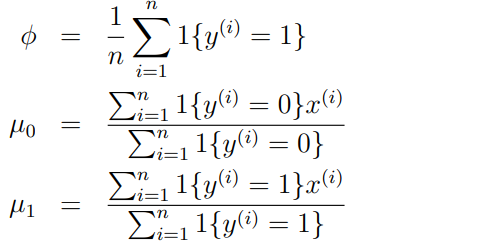
\includegraphics[width=0.5\textwidth]{figs/2.png}
      \label{2}
    \end{figure}
    \item برای ایجاد شهود پیرامون مقدار $\mu_0$ و $\mu_1$ که مقدار فرمول را به حداکثر می‌رساند، به این فکر کنید که تخمین حداکثر $likelihood$ میانگین همه ویژگی‌ها برای یک کلاس خاص، مثلاً تومورهای خوش‌خیم، که با برچسب کلاس $0$ در مجموعه داده ما نشان داده می‌شود، چقدر خواهد بود.

    $\mu_0$ را در نظر بگیرید. یک راه معقول برای تخمین $\mu_0$ این است که تمام تومورهای خوش خیم $training\:set$ خود را در نظر بگیرید (همه نمونه های منفی، یعنی ورودی ها به صورت 0) و فقط میانگین ویژگی های آنها را در نظر بگیرید. معادله فوق راهی برای نوشتن این شهود است. صورت کسر مجموع بردارهای ویژگی برای همه نمونه های تومورهای خوش خیم در $training\:set$ است (یعنی نمونه هایی با $y=0$) در حالی که مخرج به سادگی تعداد تومورهای خوش خیم در مجموعه آموزشی است.


\end{itemize}


البته بدیهتا وقتی $y$ را میدانیم(از $observation$) با توجه به ستینگ احتمالاتی ما دیگه پارامتر های دیگر توضیع رو نیاز نداریم و توضیع پارامتر $class\:conditional$ هم وجودش معنایی ندارد.

\subsection*{مورد خاص: $\Sigma_{k}=\sigma^{2}I$ }
شکل بالا$training\:set$، و همچنین خطوط دو توزیع گاوسی که با داده های هر یک از دو کلاس مطابقت دارند را نشان میدهد. توجه داشته باشید که دو توضیع گاوسی ماتریس کوواریانس $\Sigma$ مشترک دارند ولی $\mu$ های متفاوت.

همچنین فرض داریم که $p(y=1|x) = 0.5$

\begin{figure}[h]
  \centering
  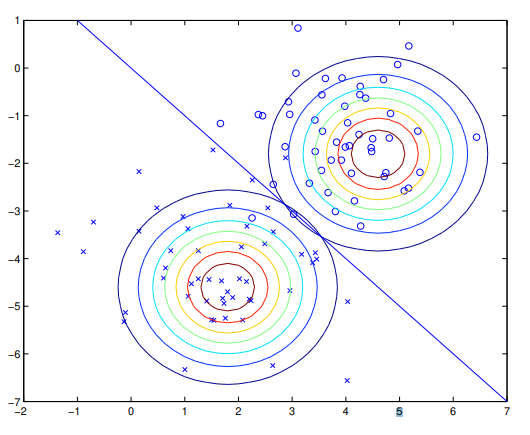
\includegraphics[width=0.7\textwidth]{figs/3.png}
  \caption{حالت خاص $\Sigma$ برابر}
  \label{3}
\end{figure}

در این حالت خاص مرز تصمیم معمولاً در نقطه میانی بین دو مرکز کلاس قرار دارد، که منعکس کننده احتمال برابر برای هر کلاس است. این نشان دهنده نقطه ای است که هر دو کلاس به یک اندازه محتمل هستند و به عنوان جداکننده بین آنها عمل می کند و در نهایت یک تابع درجه 1 است.

به طور ساده میشود گفت که چون $prior$ ها مساوی اند $posterior$ برابر $likelihood$ است و دلیل وسط قرار گرفتن خط همین بود که در آن وسط $posterior$ ها هم همدیگر را قطع میکردند.



حال فرض کنیم که $prior$ کلاس سیاه بیشتر هست در این صورت مرز به سمت قرمز میرود. در واقع تمایل به قرار گیری در کلاس سیاه بیشتر میشود به دلیل $prior$.

\newpage
\begin{figure}[h]
  \centering
  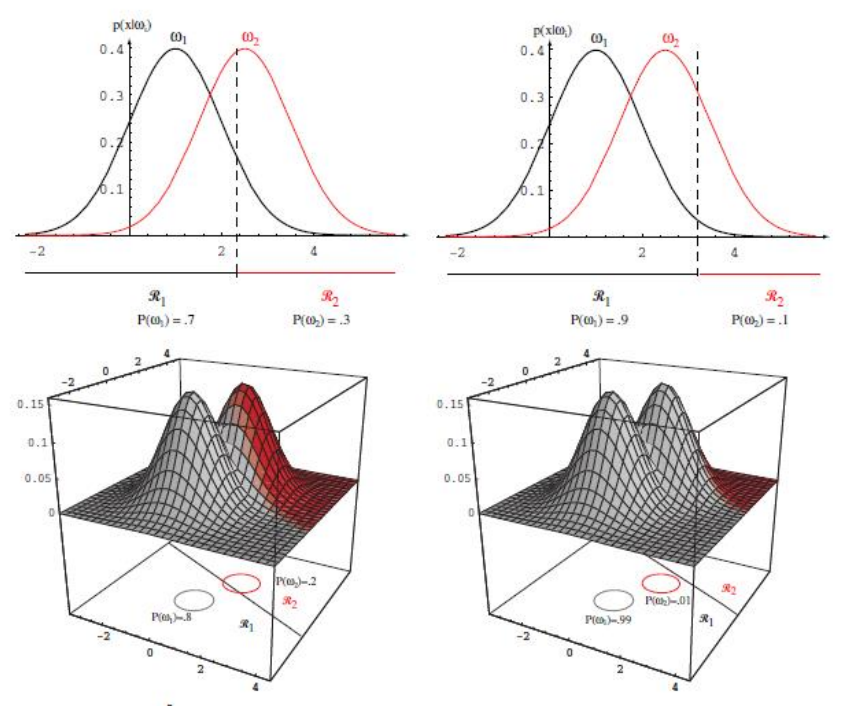
\includegraphics[width=0.7\textwidth]{figs/4.png}
  \caption{حالت خاص $\Sigma$ برابر}
  \label{4}
\end{figure} 


\subsection*{مورد خاص: $\Sigma_{k}=\Sigma$ }

در این حالت برای توزیع های گاوسی ای را داریم با ماتریس کواریانس های مساوی ولی دلخواه. ابرصفحه های تصمیم ما در این حالت خاص $GDA$ معادل رویکرد $LDA$ است.
و اینکه ابرصفحه های تصمیم نباید بر خطی که میانه کلاس ها را به هم وصل می کند عمود باشند.
\begin{figure}[h]
  \centering
  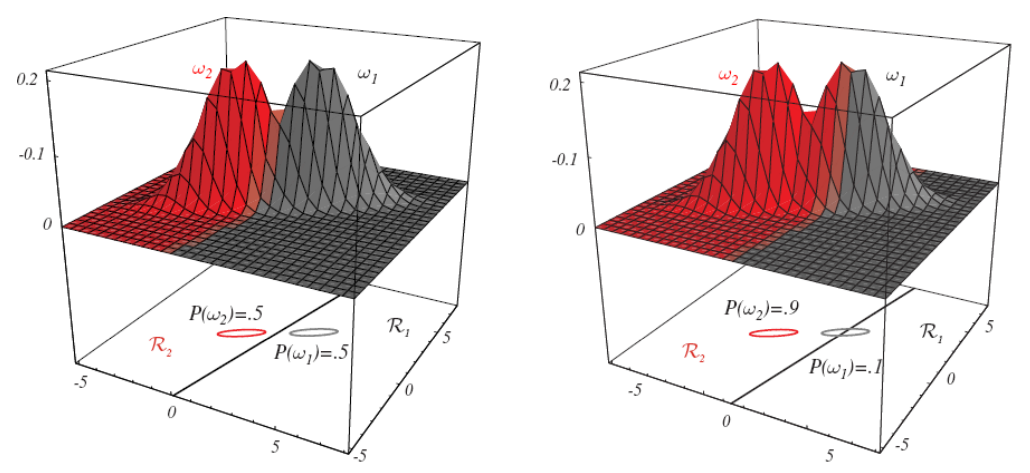
\includegraphics[width=0.75\textwidth]{figs/5.png}
  \caption{حالت خاص $\Sigma_{k}=\Sigma$}
  \label{5}
\end{figure}


\section*{$Naïve\:Bayes\:classifier$}
در $GDA$، بردارهای ویژگی $x$ بردارهای پیوسته و $real-valued$ بودند. بیایید اکنون در مورد یک الگوریتم یادگیری متفاوت صحبت کنیم که در آن $x_j$ ها گسسته ارزیابی می شوند.
برای مثال، ساخت فیلتر $spam$ ایمیل را با استفاده از $ML$ در نظر بگیرید. در اینجا، می‌خواهیم پیام‌ها را بر اساس ایمیل‌های تجاری ناخواسته ($spam$) یا $non-spam$ طبقه‌بندی کنیم. پس از یادگیری انجام این کار، می‌توانیم ایمیل‌خوان خود را به‌طور خودکار پیام‌های $spam$ را فیلتر کرده و شاید آنها را در یک پوشه ایمیل جداگانه قرار دهیم. طبقه بندی ایمیل ها نمونه ای از مجموعه وسیع تری از مشکلات به نام طبقه بندی متن است.
فرض کنید یک $ training\:set$ داریم (مجموعه ای از ایمیل ها که به عنوان $spam$ یا $non-spam$ برچسب گذاری شده اند). ما ساخت فیلتر $spam$ خود را با مشخص کردن ویژگی‌هایی که $x_j$ برای نمایش ایمیل استفاده می‌شود، آغاز می‌کنیم.
ما یک ایمیل را از طریق یک بردار ویژگی نشان خواهیم داد که طول آن برابر با تعداد کلمات در فرهنگ لغت است. به طور خاص، اگر یک ایمیل حاوی کلمه $j$-ام فرهنگ لغت باشد، $x_j$ = 1 را تنظیم می کنیم. در غیر این صورت، اجازه می دهیم $x_j$ = 0. برای مثال، بردار
\begin{figure}[h]
  \centering
  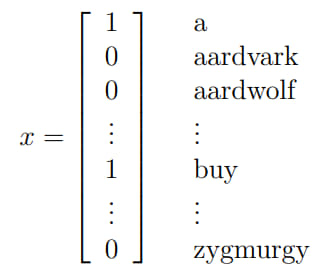
\includegraphics[width=0.5\textwidth]{figs/7.png}
  \label{7}
\end{figure}
برای نشان دادن ایمیلی استفاده می شود که حاوی کلمات "$a$" و "$buy$" است، اما نه "$aardvark$"، "$aardwolf$" یا "$zygmurgy$". مجموعه کلماتی که در بردار ویژگی کدگذاری شده اند، واژگان نامیده می شود. بنابراین بعد $x$ برابر با اندازه واژگان است.
با انتخاب بردار ویژگی خود، اکنون می خواهیم یک مدل $generative$ بسازیم. بنابراین، باید $p(x|y)$ را مدل کنیم. اما اگر مثلاً واژگانی متشکل از 50000 کلمه داشته باشیم، آنگاه
 $x ∈ {0، 1}^50000$ ($x$ یک بردار 50000 بعدی از 0 و 1 است)، و اگر بخواهیم $x$ را به طور صریح با توزیع $multinomial$ بر روی $2^50000$ نتیجه ممکن مدل کنیم، سپس ما به یک بردار پارامتر $(2^50000-1)$ بعدی خواهیم رسید. این به وضوح تعداد پارامترهای زیادی است.
 
 بنابراین برای مدل کردن $p(x|y)$، به یک فرض نیاز خواهیم داشت.
یک فرضی وجود دارد به نام فرض $Naïve\:Bayes$ که میگوید با فرض کلاس، فیچر ها مستقل از هم تولید میشوند:
\begin{figure}[h]
  \centering
  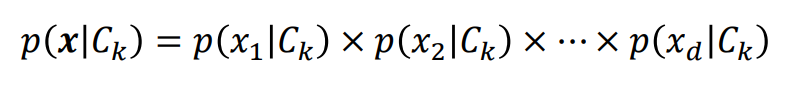
\includegraphics[width=0.55\textwidth]{figs/6.png}
  \label{6}
\end{figure}

پس وقتی یک


\end{document}
